% $HeadURL$

\subsection{Glyph: \glyph{Unit of information}}
\label{sec:unitInfo}

When representing biological entities, it is often necessary to convey some abstract information about the entity's function that cannot (or does not need to) be easily related to its structure.
The \glyph{unit of information} is a decoration that can be used in this situation to add information to a glyph.
Some example uses include: characterising a logical part of an entity such as a functional domain (a binding domain, a catalytic site, a promoter, etc.), or the information encoded in the entity (an exon, an open reading frame, etc.).
A \glyph{unit of information} can also convey information about the physical environment, or the specific type of biological entity it is decorating.

\begin{glyphDescription}

\glyphSboTerm
Not applicable.

\add{
\glyphIncoming
None.
}

\add{
\glyphOutgoing
None.
}

\glyphContainer
A \glyph{unit of information} is represented by a rectangular shape, as shown in \fig{unitInfo}.
\corr{The long side of the rectangle should be oriented parallel to the border of the \glyph{EPN} being annotated by the \glyph{unit of information}.}{}
\rougny{That is a complicated requirement. It would require to be able to draw vertical text. Also, it is for example not required for arcs' units of information in PD. I would drop it.
UD: I agree.
AR: dropped it}
The centre of the \corr{\glyph{unit of information}}{shape} should be placed on the \corr{mid-line of the}{}border of the \glyph{EPN}.
% \rougny{I am not sure this is correct. Does this mean it should be at the mid-point of the border?
% We could replace this sentence and the previous one by: ``the centre of the shape should be placed on the border of the EPN''.
% VT: I thing the rephrasing better indeed.
% UD: I agree.}

\glyphLabel
A \glyph{unit of information} is identified by a label that is \corr{an unbordered box containing}{} a string of characters \corr{.
The characters}{that} may be distributed on several lines to improve readability.
The centre of the label must be placed on the centre of the \corr{shape}{container}.
The label may extend outside of the \corr{shape}{container}.
\corr{The text of the label defines the information carried by the\glyph{unit of information}.}{} \blinov{Obvious. Remove.} 
For certain predefined types of information having controlled vocabularies associated with them, SBGN defines specific prefixes that must be included in the text of the label and associated with the \corr{prefix}{information's value} to indicate the type of information in question. Together, a prefix and a value constitute the label. The controlled vocabularies predefined in \SBGNPDLone are described in \sect{CVs} and summarised in the following list:

\begin{center}
  \begin{itemize}\setlength{\parskip}{0ex}
  \item[\texttt{pc}] container physical characteristic
  \item[\texttt{mt}] entity pool material type
  \item[\texttt{ct}] entity pool conceptual type
  \item[\texttt{N}]  multimer cardinality
  \end{itemize}
  \draeger{What happens if one wants to have multiple such characteristics, \eg a multimer cardinality in combination with a material entity? Vasundra says: I guess they create multiple units of information, one for each characteristic wanted? Adrien: I would say the same as Vasundra.}
\end{center}

\glyphAux
\corr{A \glyph{unit of information} does not carry any auxiliary items.}{None.}

\end{glyphDescription}

\begin{figure}[H]
  \centering
  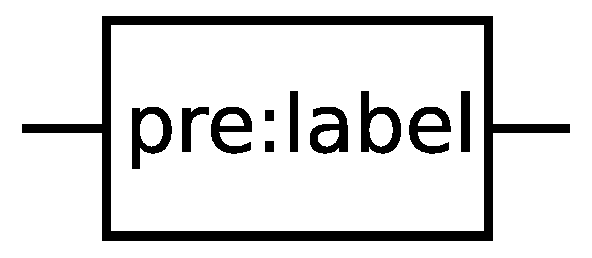
\includegraphics{images/unitInformation}
  \caption{The \PD glyph for \glyph{unit of information}, shown plain on the left, and decorating a \glyph{macromolecule} (\sect{macromolecule}) on the right.}
  \label{fig:unitInfo}
\end{figure}

% The following is for [X]Emacs users.   Please leave in place.
% Local Variables:
% TeX-master: "../sbgn_PD-level1"
% End:
